\documentclass[notes,blackandwhite,mathsans]{beamer}

\usepackage{amsmath}
\usepackage{amssymb}
\usepackage{graphicx}
\usepackage{fancybox}
\usepackage{booktabs}
\usepackage{multirow,pxfonts}
\usepackage{cmbright}
\usepackage{color}
\usepackage{xcolor}
\usepackage{enumitem}
\usepackage{animate}
\usepackage{changepage}

\usepackage[T1]{fontenc}
\fontencoding{T1}  
\usepackage[utf8]{inputenc}


\usefonttheme{default}
\setbeamercovered{invisible}
\beamertemplatenavigationsymbolsempty

\makeatletter
\setbeamertemplate{footline}
{
  \leavevmode
  \hbox{
  \begin{beamercolorbox}[wd=0.97\paperwidth,ht=2.25ex,dp=2ex,right]{}
{\color{mcxs2} \insertframenumber{} / \inserttotalframenumber}
  \end{beamercolorbox}}%
}




\definecolor{mcxs1}{HTML}{05386B}
\definecolor{mcxs2}{HTML}{379683}
\definecolor{mcxs3}{HTML}{5CDB95}
\definecolor{mcxs4}{HTML}{8EE4AF}
\definecolor{mcxs5}{HTML}{EDF5E1}
\setbeamercolor{frametitle}{fg=mcxs2}
\AtBeginDocument{\color{mcxs1}}

%\setbeamercolor{itemize text}{fg=mcxs5}
\setbeamercolor{itemize item}{fg=mcxs1}
\setbeamercolor{itemize subitem}{fg=mcxs2}
\setbeamercolor{enumerate item}{fg=mcxs1}
\setbeamercolor{description item}{fg=mcxs1}

\setbeamertemplate{itemize item}[triangle]
\setbeamertemplate{itemize subitem}[circle]




\begin{document}
%\fontfamily{pag}\selectfont
%\setbeamerfont{title}{family=\fontfamily{pag}\selectfont}
%\setbeamerfont{frametitle}{family=\fontfamily{pag}\selectfont}
%\setbeamerfont{framesubtitle}{family=\fontfamily{pag}\selectfont}




\begin{frame}
\centering
\includegraphics[scale=1.87]{mcxs.png}
\end{frame}





{\setbeamercolor{background canvas}{bg=mcxs4}
\begin{frame}

\vspace{1cm}
\begin{tabular}{rl}
&\textbf{\LARGE\color{mcxs1} Macroeconometrics}\\[8ex]
\textbf{\Large\color{mcxs5} Lecture 4}&\textbf{\Large\color{mcxs2}Numerical optimization and}\\
&\textbf{\Large\color{mcxs2}integration}\\[17ex]
&\textbf{\color{mcxs2}Tomasz Wo\'zniak}\\[1ex]
&{\small\color{mcxs5} Department of Economics}\\
&{\small\color{mcxs5}University of Melbourne}
\end{tabular}

\end{frame}
}





{\setbeamercolor{background canvas}{bg=mcxs4}
\begin{frame}

\vspace{1cm} \textbf{\color{mcxs1}Numerical optimization}

\bigskip\textbf{\color{mcxs2}Numerical integration}

%\vspace{1cm} Useful readings: \\ \footnotesize
%\smallskip{\color{mcxs2}Harris, Hurn, \& Martin (2012) Chapter 3: Numerical Estimation Methods, Econometric Modelling with Time Series
%
%\smallskip\noindent Greenberg (2008) Chapter 7: Simulation by MCMC Methods,\\ Introduction to Bayesian Econometrics}

\bigskip\normalsize Materials:\\ \footnotesize
{\color{mcxs2}Wo\'zniak (2021) Posterior derivations for a simple linear regression model, Lecture notes}\\
{\color{mcxs2}An R file} \texttt{L4 mcxs.R} {\color{mcxs2}for the reproduction the results}

\end{frame}
}





%{\setbeamercolor{background canvas}{bg=mcxs4}
%\begin{frame}
%
%\bigskip\textbf{\color{mcxs1}Objectives.}
%\begin{itemize}[label=$\blacktriangleright$]
%\item {\color{mcxs1}To introduce core techniques for statistical inference}
%\item {\color{mcxs1}To understand the workings of numerical algorithms}
%\item {\color{mcxs1}To learn to recognize usable outputs}
%\end{itemize}
%
%\bigskip\textbf{\color{mcxs2}Learning outcomes.}
%\begin{itemize}[label=$\blacktriangleright$]
%\item {\color{mcxs2}Using Newton-Raphson and BHHH methods for numerical optimization}
%\item {\color{mcxs2}Using Gibbs sampler for numerical integration}
%\item {\color{mcxs2}Manipulating algorithm parameters to obtain reliable outcomes}
%\end{itemize}
%
%\end{frame}
%}





{\setbeamercolor{background canvas}{bg=mcxs4}
\begin{frame}

\begin{adjustwidth}{-0.5cm}{0cm}
%\FlushLeft
\vspace{7.3cm}\Large
\textbf{{\color{mcxs1}Numerical optimization}}\\ 
{\color{mcxs5}Maximizing the log-likelihood function}
\end{adjustwidth}

\end{frame}
}




\begin{frame}
\frametitle{Numerical optimization}

\textbf{Motivation.}

{\color{mcxs2}For many econometric models the MLE cannot be found analytically as the system of equations for the first order conditions cannot or is difficult to solve.}
$$ G\left(\hat\theta\right) = \mathbf{0} $$

{\color{mcxs2}In such cases, we rely on numerical optimization methods that potentially give an approximate solution to the problem above that is as close to the exact solution as possible or required.}

\end{frame}





\begin{frame}
\frametitle{Numerical optimization: the idea}



\smallskip{\color{mcxs2}Use an algorithm that requires:}
\begin{description}
\item[starting values] {\color{mcxs2}for the parameter vector, denoted by} $\theta_{(0)}${\color{mcxs2}, at which the algorithm begins the search of the solution}
\item[a dynamic rule] {\color{mcxs2}that generates values of parameters in subsequent iterations of the algorithm, denoted by} $\theta_{(k)}${\color{mcxs2}, that are closer and closer to the solution}
\item[a stopping rule] {\color{mcxs2}that stops the algorithm at a point that is close enough to the solution given the required precision}
\end{description}

\end{frame}


\begin{frame}
\frametitle{Numerical optimization: starting values}


\smallskip{\color{mcxs2}Are usually generated from:}
\begin{description}
\item[preliminary data analysis] {\color{mcxs2}some summary statistics can be informative about approximate values of the parameters}
\item[a simplified model] {\color{mcxs2}that can be easily estimated using a simpler method}
\item[a grid of admissible values] {\color{mcxs2}that is a robust way of searching for the global maximum (away from a boundary of the parameter space) in cases where the solutions provided by algorithm are sensitive to starting values}
\end{description}


\end{frame}






\begin{frame}
\frametitle{Numerical optimization: Newton-Raphson method}

\vspace{1cm}
$$ \theta_{(k)} = \theta_{(k-1)} - H^{-1}\left(\theta_{(k-1)}\right)G\left(\theta_{(k-1)}\right) $$

\bigskip\begin{description}
\item[$\theta_{(k)}$] {\color{mcxs2}-- value of parameters in the current step of the algorithm}
\item[$\theta_{(k-1)}$] {\color{mcxs2}-- value of parameters in the previous step of the algorithm}
\item[$H^{-1}\left(\theta_{(k-1)}\right)$] {\color{mcxs2}-- inverse of Hessian matrix evaluated at} $\theta_{(k-1)}$
\item[$G\left(\theta_{(k-1)}\right)$] {\color{mcxs2}-- the gradient vector evaluated at} $\theta_{(k-1)}$
\end{description}

\end{frame}





\begin{frame}
\frametitle{Numerical optimization: Newton-Raphson method}

\textbf{Gradient vector and Hessian matrix} {\color{mcxs2}are computed using:}
\bigskip\begin{description}
\item[analytical formulae] {\color{mcxs2}-- provided by the user}
\item[numerical approximation] {\color{mcxs2}-- which is the default option in existing software packages, it is also time-consuming}
\item[automatic differentiation] {\color{mcxs2}-- where the exact derivatives of the objective function are computed using designated software\\ -- no existing software packages offer this functionality}
\end{description}

\end{frame}





\begin{frame}
\frametitle{Numerical optimization: BHHH method}

{\color{mcxs2}Based on} Brendt, Hall, Hall, Hausman (1974)

\begin{align*} 
\theta_{(k)} &= \theta_{(k-1)} {\color{mcxs3}+ J^{-1}\left(\theta_{(k-1)}\right)}G\left(\theta_{(k-1)}\right)
\end{align*} 

\bigskip{\color{mcxs2}Hessian matrix ordinate} $- H^{-1}\left(\theta_{(k-1)}\right)$ {\color{mcxs2}is approximated by the outer product of gradients} {\color{mcxs3}$J^{-1}\left(\theta_{(k-1)}\right)$}.

\small
\begin{align*} 
{\color{mcxs3}J\left(\theta_{(k-1)}\right)} &= {\color{mcxs2}\frac{1}{T}\sum_{t=1}^{T}}g_t\left(\theta_{(k-1)}\right)g_t\left(\theta_{(k-1)}\right)'\\
g_t\left(\theta_{(k-1)}\right) &= {\color{mcxs2}\frac{\partial l(y_t|x_t,\theta)}{\partial\theta}\big|_{\theta=\theta_{(k-1)}}}
\end{align*} 

\end{frame}





\begin{frame}{Numerical optimization: stopping rules}

{\color{mcxs2}Let} $\epsilon$ {\color{mcxs2}be a small positive number.}
\begin{description}
\item[$\epsilon=\mathtt{1e-06}$] {\color{mcxs2}-- for preliminary estimations}
\item[$\epsilon<\mathtt{1e-08}$] {\color{mcxs2}-- for reporting final results}
\end{description}

\bigskip\textbf{Stopping rules.}\\
{\color{mcxs2}Stop the algorithm when either of the criterion holds:}
\begin{description}
\item[$\big|G\left(\theta_{(k)}\right)\big|<\epsilon$] {\color{mcxs2}-- related directly to absolute value of gradient}
\item[$\big|\big|\theta_{(k)} - \theta_{(k-1)}\big|\big|<\epsilon$] {\color{mcxs2}-- an increment in parameter values over iterations is negligible, where $||\cdot||$ is some norm, e.g., a~maximum value of elements of vector }
\item[$k>k_{max}$] {\color{mcxs2}-- a rule thanks to which we avoid running the computations for a long time without achieving convergence. This might happen when we set $\epsilon$ to too small a value. This rule should not be binding for the final results. }
\end{description}

\bigskip{\color{mcxs1}Always check the message regarding the convergence!}

\end{frame}






\begin{frame}
\frametitle{Numerical optimization: illustration}

\textbf{A simple linear regression model} with known slope $\beta=1$
\begin{align*} 
Y &= X + E\\
E|X &\sim\mathcal{N}\left(\mathbf{0}_T, {\color{mcxs3}\sigma^2}I_T\right)\\
\downarrow &\\
Y|X,\beta=1 &\sim\mathcal{N}\left( X, {\color{mcxs3}\sigma^2}I_T\right)
\end{align*} 

\bigskip\textbf{The log-likelihood function.}
\begin{equation*}
l\left({\color{mcxs3}\sigma^2}|Y,X\right) = {\color{mcxs2}-\frac{T}{2}\log(2\pi)} -\frac{T}{2}\log\left({\color{mcxs3}\sigma^2}\right)  -\frac{1}{2}\frac{1}{{\color{mcxs3}\sigma^2}}(Y-X)'(Y- X) 
\end{equation*}

\bigskip\textbf{MLE:} $ \hat\sigma^2 = \frac{1}{T}(Y-X)'(Y-X) = \frac{1}{T}E'E $

\end{frame}



\begin{frame}{Numerical optimization: illustration}

\bigskip\textbf{Derivatives.}
\begin{align*}
G\left({\color{mcxs3}\sigma^2}\right) &= -\frac{T}{2}\frac{1}{\sigma^2} + \frac{1}{2}\frac{E'E}{\left( \sigma^2\right)^2}\\
{\color{mcxs2}g_t\left({\color{mcxs3}\sigma^2}\right)} &= {\color{mcxs2}-\frac{T}{2}\frac{1}{\sigma^2} + \frac{1}{2}\frac{(y_t-x_t)^2}{\left( \sigma^2\right)^2}} \\
H\left({\color{mcxs3}\sigma^2}\right) &= \frac{T}{2}\frac{1}{\left(\sigma^2\right)^2} - \frac{E'E}{\left( \sigma^2\right)^3}
\end{align*}

\bigskip\textbf{Newton-Raphson rule.}\footnotesize
\begin{align*} 
\sigma^2_{(k)} &= \sigma^2_{(k-1)} + \left[ \frac{E'E}{\left( \sigma^2_{(k-1)}\right)^3} - \frac{T}{2}\frac{1}{\left(\sigma^2_{(k-1)}\right)^2}  \right]^{-1}\left[ \frac{1}{2}\frac{E'E}{\left( \sigma^2_{(k-1)}\right)^2}-\frac{T}{2}\frac{1}{\sigma^2_{(k-1)}} \right]\\[1ex]
&= \sigma^2_{(k-1)} + \sigma^2_{(k-1)}\left[2E'E - T\sigma^2_{(k-1)} \right]^{-1}\left[ E'E - T\sigma^2_{(k-1)} \right]\\
\end{align*}

\end{frame}

{\setbeamercolor{background canvas}{bg=mcxs4}
\begin{frame}{Numerical optimization: illustration}
  \animategraphics[loop,controls,width=\linewidth]{1}{./grphs/newton-raphson-}{1}{9}
\end{frame}
}


\begin{frame}{Numerical optimization: illustration}

\textbf{Data for the animation.}\tiny
\begin{center}
\begin{tabular}{ccccccc}
\toprule
$k$ & $\sigma^2_{(k)}$ & $l(\sigma^2_{(k)}|Y,X)$ & $|G(\sigma^2_{(k)})|$ & $|G(\sigma^2_{(k)})|<\epsilon$ &  $|\sigma^2_{(k)}-\sigma^2_{(k-1)}|$ & $|\sigma^2_{(k)}-\sigma^2_{(k-1)}|<\epsilon$\\
\midrule
1&    0.500& -249.287& 284.1&     FALSE&           0.213&                 FALSE\\
2 &   0.713& -209.707& 118.9&     FALSE&           0.275&                 FALSE\\
3&    0.988& -188.495&  47.8&     FALSE&           0.323&                 FALSE\\
4&    1.311& -178.686&  17.6&     FALSE&           0.316&                 FALSE\\
5&    1.627& -175.253&   5.6&     FALSE&           0.216&                 FALSE\\
6&    1.842& -174.567&   1.1&     FALSE&           0.072&                 FALSE\\
7&    1.9144& -174.523&   0.08&     FALSE&           0.006&                 FALSE\\
8&    1.9205& -174.523&   0.001&     FALSE&           0.000&                 FALSE\\
9&    1.9205& -174.523&   0.000&     TRUE&           0.000&                 TRUE\\
\bottomrule
\end{tabular}\\
$ \hat\sigma^2 =  1.9205, \qquad \epsilon = 10^{-6}$
\end{center}

\end{frame}




{\setbeamercolor{background canvas}{bg=mcxs4}
\begin{frame}

\begin{adjustwidth}{-0.5cm}{0cm}
%\FlushLeft
\vspace{8.3cm}\Large
\textbf{{\color{mcxs2}Numerical integration} {\color{mcxs5}Gibbs sampler}}
\end{adjustwidth}

\end{frame}
}




\begin{frame}{Numerical integration}

\textbf{Motivation.}

{\color{mcxs2}For most of econometric models analytical derivation of the joint posterior distribution of the parameters is impossible. The distribution is known only up to its kernel:}
$$ p(\theta|Y)\propto L(\theta|Y)p(\theta) $$
{\color{mcxs2}In such cases, we use numerical integration algorithms from the family of Monte Carlo Markov Chain (MCMC) methods to generate random draws from the joint posterior distribution and we use them to compute all of the required characteristics of this distribution.\\

\smallskip Gibbs sampler is an MCMC algorithm that is feasible for most of the models discussed in this subject. }

\end{frame}



\begin{frame}{Gibbs sampler}

\textbf{Idea for the algorithm.}

{\color{mcxs2} Suppose that the parameters can be conveniently divided in two groups:} $\theta=(\theta_1, \theta_2)$.

\bigskip{\color{mcxs2}For many models, when the joint posterior distribution} $p(\theta_1, \theta_2|Y)$ {\color{mcxs2}cannot be derived, the} {\color{mcxs3}full conditional posterior distributions}, $p(\theta_1|Y,\theta_2)$ {\color{mcxs2}and} $p(\theta_2|Y,\theta_1)${\color{mcxs2}, are available.}

\end{frame}






\begin{frame}{Gibbs sampler}

\textbf{Construction of the algorithm.}

\small
\bigskip\begin{description}
\item[Initialize] $\theta_2$ {\color{mcxs2}at} $\theta_2^{(0)}$
\item[At each iteration] $s$:
\begin{description}
\item[1. Draw] {\color{mcxs2}a random number/vector from} $\theta_1^{(s)}\sim p\left(\theta_1|Y,\theta_2^{(s-1)}\right)$

\smallskip\item[2. Draw] {\color{mcxs2}a random number/vector from} $\theta_2^{(s)}\sim p\left(\theta_2|Y,\theta_1^{(s)}\right)$
\end{description}
\item[Repeat] {\color{mcxs2}steps} 1. {\color{mcxs2}and} 2. $S_1 + S_2$ {\color{mcxs2}times}
\item[Discard] {\color{mcxs2}the first} $S_1$ {\color{mcxs2}draws that allowed the algorithm to} {\color{mcxs3}converge to the stationary posterior distribution}
\item[Output] {\color{mcxs2}is a sample of draws from the joint posterior distribution} $\left\{ \theta_1^{(s)}, \theta_2^{(s)} \right\}_{s=S_1+1}^{S_1 + S_2}$
\end{description}

\end{frame}






\begin{frame}{A simple linear regression model}

\begin{align*} 
Y &= \beta X + E\\
E|X &\sim\mathcal{N}\left(\mathbf{0}_T, \sigma^2I_T\right)\\
\downarrow &\\
Y|X &\sim\mathcal{N}\left(\beta X, \sigma^2I_T\right)
\end{align*} 

\bigskip\textbf{The likelihood function.}
\begin{equation*}
L\left(\theta|Y,X\right) = {\color{mcxs2}(2\pi)^{-\frac{T}{2}}} \left( {\color{mcxs3}\sigma^2} \right)^{-\frac{T}{2}}\exp\left\{ -\frac{1}{2}\frac{1}{\color{mcxs3}\sigma^2}(Y-{\color{mcxs3}\beta} X)'(Y-{\color{mcxs3}\beta} X) \right\}
\end{equation*}


\end{frame}







\begin{frame}
\frametitle{Conditionally-conjugate prior distribution}

{\color{mcxs2}A conditionally-conjugate prior distribution leads to the full conditional posterior distribution of the same form.}

\bigskip{\color{mcxs2}Let} $({\color{mcxs3}\beta,\sigma^2})$ {\color{mcxs2}follow an independent normal and inverse gamma 2 distribution:}
\begin{align*}
p\left({\color{mcxs3}\beta}, {\color{mcxs3}\sigma^2}\right) &= p\left({\color{mcxs3}\beta}\right)p\left({\color{mcxs3}\sigma^2}\right)\\[1ex]
p\left({\color{mcxs3}\beta}\right)&=\mathcal{N}\left( \underline{\beta}, \underline{\sigma}_{\beta}^2 \right)\\
p\left({\color{mcxs3}\sigma^2}\right)&=\mathcal{IG}2(\underline{s},\underline{\nu})
\end{align*}

\smallskip\textbf{pdf.}
\begin{equation*} 
p\left({\color{mcxs3}\beta}, {\color{mcxs3}\sigma^2}\right) \propto 
\exp\left\{ -\frac{1}{2}\frac{1}{\underline{\sigma}_{\beta}^2}({\color{mcxs3}\beta}-\underline{\beta})'({\color{mcxs3}\beta}-\underline{\beta}) \right\} \times
\left({\color{mcxs3}\sigma^2}\right)^{-\frac{\underline{\nu}+2}{2}}\exp\left\{ -\frac{1}{2}\frac{\underline{s}}{{\color{mcxs3}\sigma^2}} \right\}
\end{equation*} 
\end{frame}




\begin{frame}
\frametitle{Derive Gibbs sampler}

\textbf{Full conditional posterior distribution of {\color{mcxs3}$\beta$}:} $p\left({\color{mcxs3}\beta}|Y,X,\sigma^2\right)$
{\color{mcxs2}Conditioning on} $\sigma^2$ {\color{mcxs2}implies that for the sake of deriving the full conditional posterior distribution of} {\color{mcxs3}$\beta$} {\color{mcxs2}we treat it as non-random.}

\bigskip\textbf{Bayes' rule.}
$$ p\left({\color{mcxs3}\beta}|Y,X,\sigma^2\right) \propto L\left({\color{mcxs3}\beta},\sigma^2|Y,X\right)p\left({\color{mcxs3}\beta}\right) $$

\bigskip\textbf{kernel of the full conditional distribution.}\footnotesize
\begin{equation*} 
p\left({\color{mcxs3}\beta}|Y,X,\sigma^2\right) \propto \exp\left\{ -\frac{1}{2}\frac{1}{\sigma^2}(Y-{\color{mcxs3}\beta} X)'(Y-{\color{mcxs3}\beta} X) \right\} \times
\exp\left\{ -\frac{1}{2}\frac{1}{\underline{\sigma}_{\beta}^2}({\color{mcxs3}\beta}-\underline{\beta})'({\color{mcxs3}\beta}-\underline{\beta}) \right\}
\end{equation*} 
\end{frame}





\begin{frame}
\frametitle{Derive Gibbs sampler}

\textbf{Full conditional posterior distribution of {\color{mcxs3}$\beta$}:} $p\left({\color{mcxs3}\beta}|Y,X,\sigma^2\right)$
\footnotesize
\begin{align*} 
p\left({\color{mcxs3}\beta}|Y,X,\sigma^2\right) &\propto \exp\left\{ -\frac{1}{2}\frac{1}{\sigma^2}(Y-{\color{mcxs3}\beta} X)'(Y-{\color{mcxs3}\beta} X) \right\} \exp\left\{ -\frac{1}{2}\frac{1}{\underline{\sigma}_{\beta}^2}({\color{mcxs3}\beta}-\underline{\beta})'({\color{mcxs3}\beta}-\underline{\beta}) \right\}\\
&= \exp\left\{ -\frac{1}{2}\left[\frac{1}{\sigma^2}(Y-{\color{mcxs3}\beta} X)'(Y-{\color{mcxs3}\beta} X) + \frac{1}{\underline{\sigma}_{\beta}^2}({\color{mcxs3}\beta}-\underline{\beta})'({\color{mcxs3}\beta}-\underline{\beta}) \right]\right\}\\
&= \exp\left\{ -\frac{1}{2}\left[
{\color{mcxs3}\beta}^2\left( \underline{\sigma}_{\beta}^{-2}+ \sigma^{-2}X'X \right) - {\color{mcxs3}\beta}2\left( 
\underline{\sigma}_{\beta}^{-2}\underline{\beta} + \sigma^{-2}X'Y 
\right) + \dots \right]\right\}
\end{align*} 

\bigskip\normalsize{\color{mcxs2}Which is in a form of a normal distribution.}
\end{frame}



\begin{frame}
\frametitle{Derive Gibbs sampler}

\textbf{Full conditional posterior distribution of {\color{mcxs3}$\beta$}:} $p\left({\color{mcxs3}\beta}|Y,X,\sigma^2\right)$
\begin{align*} 
p\left({\color{mcxs3}\beta}|Y,X,\sigma^2\right) &=\mathcal{N}\left(\overline{\beta}, \overline{\sigma}_{\beta}^2\right)\\[3ex]
\overline{\sigma}_{\beta}^2 &= \left( \underline{\sigma}_{\beta}^{-2}+ \sigma^{-2}X'X \right)^{-1}\\[1ex]
\overline{\beta} &= \overline{\sigma}_{\beta}^2\left( \underline{\sigma}_{\beta}^{-2}\underline{\beta} + \sigma^{-2}X'Y \right)
\end{align*} 

\end{frame}







\begin{frame}
\frametitle{Derive Gibbs sampler}

\textbf{Full conditional posterior distribution of {\color{mcxs3}$\sigma^2$}:} $p\left({\color{mcxs3}\sigma^2}|Y,X,\beta\right)$
{\color{mcxs2}Conditioning on} $\beta$ {\color{mcxs2}implies that for the sake of deriving the full conditional posterior distribution of} {\color{mcxs3}$\sigma^2$} {\color{mcxs2}we treat it as non-random.}

\bigskip\textbf{Bayes' rule.}
$$ p\left({\color{mcxs3}\sigma^2}|Y,X,\beta\right) \propto L\left(\beta,{\color{mcxs3}\sigma^2}|Y,X\right)p\left({\color{mcxs3}\sigma^2}\right) $$

\bigskip\textbf{kernel of the full conditional distribution.}\footnotesize
\begin{equation*} 
p\left({\color{mcxs3}\sigma^2}|Y,X,\beta\right) \propto \left( {\color{mcxs3}\sigma^2} \right)^{-\frac{T}{2}}\exp\left\{ -\frac{1}{2}\frac{1}{\color{mcxs3}\sigma^2}(Y-\beta X)'(Y-\beta X) \right\} \times
\left({\color{mcxs3}\sigma^2}\right)^{-\frac{\underline{\nu}+2}{2}}\exp\left\{ -\frac{1}{2}\frac{\underline{s}}{{\color{mcxs3}\sigma^2}} \right\}
\end{equation*} 
\end{frame}





\begin{frame}
\frametitle{Derive Gibbs sampler}

\textbf{Full conditional posterior distribution of {\color{mcxs3}$\sigma^2$}:} $p\left({\color{mcxs3}\sigma^2}|Y,X,\beta\right)$
\footnotesize
\begin{align*} 
p\left({\color{mcxs3}\sigma^2}|Y,X,\beta\right) &\propto \left( {\color{mcxs3}\sigma^2} \right)^{-\frac{T}{2}}\exp\left\{ -\frac{1}{2}\frac{1}{\color{mcxs3}\sigma^2}(Y-\beta X)'(Y-\beta X) \right\} \times
\left({\color{mcxs3}\sigma^2}\right)^{-\frac{\underline{\nu}+2}{2}}\exp\left\{ -\frac{1}{2}\frac{\underline{s}}{{\color{mcxs3}\sigma^2}} \right\}\\
&= \left( {\color{mcxs3}\sigma^2} \right)^{-\frac{T+\underline{\nu}+2}{2}}\exp\left\{ -\frac{1}{2}\frac{1}{\color{mcxs3}\sigma^2}\left[(Y-\beta X)'(Y-\beta X) + \underline{s} \right]\right\}\\
&= \left( {\color{mcxs3}\sigma^2} \right)^{-\frac{\overline{\nu}+2}{2}}\exp\left\{ -\frac{1}{2}\frac{\overline{s}}{\color{mcxs3}\sigma^2}\right\}
\end{align*}

\bigskip\normalsize{\color{mcxs2}The final line is the kernel of the inverse gamma 2 distribution.}
 
\end{frame}



\begin{frame}
\frametitle{Derive Gibbs sampler}

\textbf{Full conditional posterior distribution of {\color{mcxs3}$\sigma^2$}:} $p\left({\color{mcxs3}\sigma^2}|Y,X,\beta\right)$

\begin{align*} 
p\left({\color{mcxs3}\sigma^2}|Y,X,\beta\right) &= \mathcal{IG}2\left( \overline{s}, \overline{\nu} \right)\\[3ex]
\overline{s} &= \underline{s} + (Y-\beta X)'(Y-\beta X) \\[1ex]
\overline{\nu} &= \underline{\nu} +T 
\end{align*}

\end{frame}




\begin{frame}
\frametitle{Gibbs sampler}

\textbf{Sampling random numbers from} $\mathcal{IG}2\left( s, \nu \right)$

\smallskip\begin{description}
\item[Step 1:] Draw {\color{mcxs2}a random number from} $\tilde{s}\sim\chi^2(\nu)$ {\color{mcxs2}using\\ R function} \texttt{rchisq()}
\item[Step 2:] Return $s/\tilde{s}$ {\color{mcxs2}as a draw from} $\mathcal{IG}2\left( s, \nu \right)$
\end{description}

\vspace{0.6cm}\textbf{Sampling random numbers from} $\mathcal{N}_1\left( \mu, \sigma^2 \right)$

\smallskip Use R function \texttt{rnorm()}

\vspace{0.6cm}\textbf{Sampling random numbers from} $\mathcal{N}_N\left( \mu, \Sigma \right)$

\smallskip Use R function \texttt{rmvnorm()} from package \texttt{mvtnorm}


\end{frame}




\begin{frame}{Gibbs sampler}

\small
\bigskip\begin{description}
\item[Initialize] $\sigma^2$ {\color{mcxs2}at} $\sigma^{2(0)}$
\item[At each iteration] $s$:
\begin{description}
\item[1. Draw] $\beta^{(s)}\sim p\left(\beta|Y,X,\sigma^{2(s-1)}\right) = \mathcal{N}\left(\overline{\beta}, \overline{\sigma}_{\beta}^2\right)$

\smallskip\item[2. Draw] $\sigma^{2(s)}\sim p\left(\sigma^2|Y,X,\beta^{(s)}\right)=\mathcal{IG}2\left( \overline{s}, \overline{\nu} \right)$
\end{description}
\item[Repeat] {\color{mcxs2}steps} 1. {\color{mcxs2}and} 2. $S_1 + S_2$ {\color{mcxs2}times}
\item[Discard] {\color{mcxs2}the first} $S_1$ {\color{mcxs2}draws that allowed the algorithm to} {\color{mcxs3}converge to the stationary posterior distribution}
\item[Output] {\color{mcxs2}is a sample of draws from the joint posterior distribution} $\left\{ \beta^{(s)}, \sigma^{2(s)} \right\}_{s=S_1+1}^{S_1 + S_2}$
\end{description}

\end{frame}





{\setbeamercolor{background canvas}{bg=mcxs4}
\begin{frame}{Gibbs sampler: illustration}
  \animategraphics[loop,controls,width=\linewidth]{4}{./grphs/Gibbs-}{1}{240}
\end{frame}
}




{\setbeamercolor{background canvas}{bg=mcxs5}
\begin{frame}{Gibbs sampler: illustration}
\centering
\textbf{Trace plots}\\
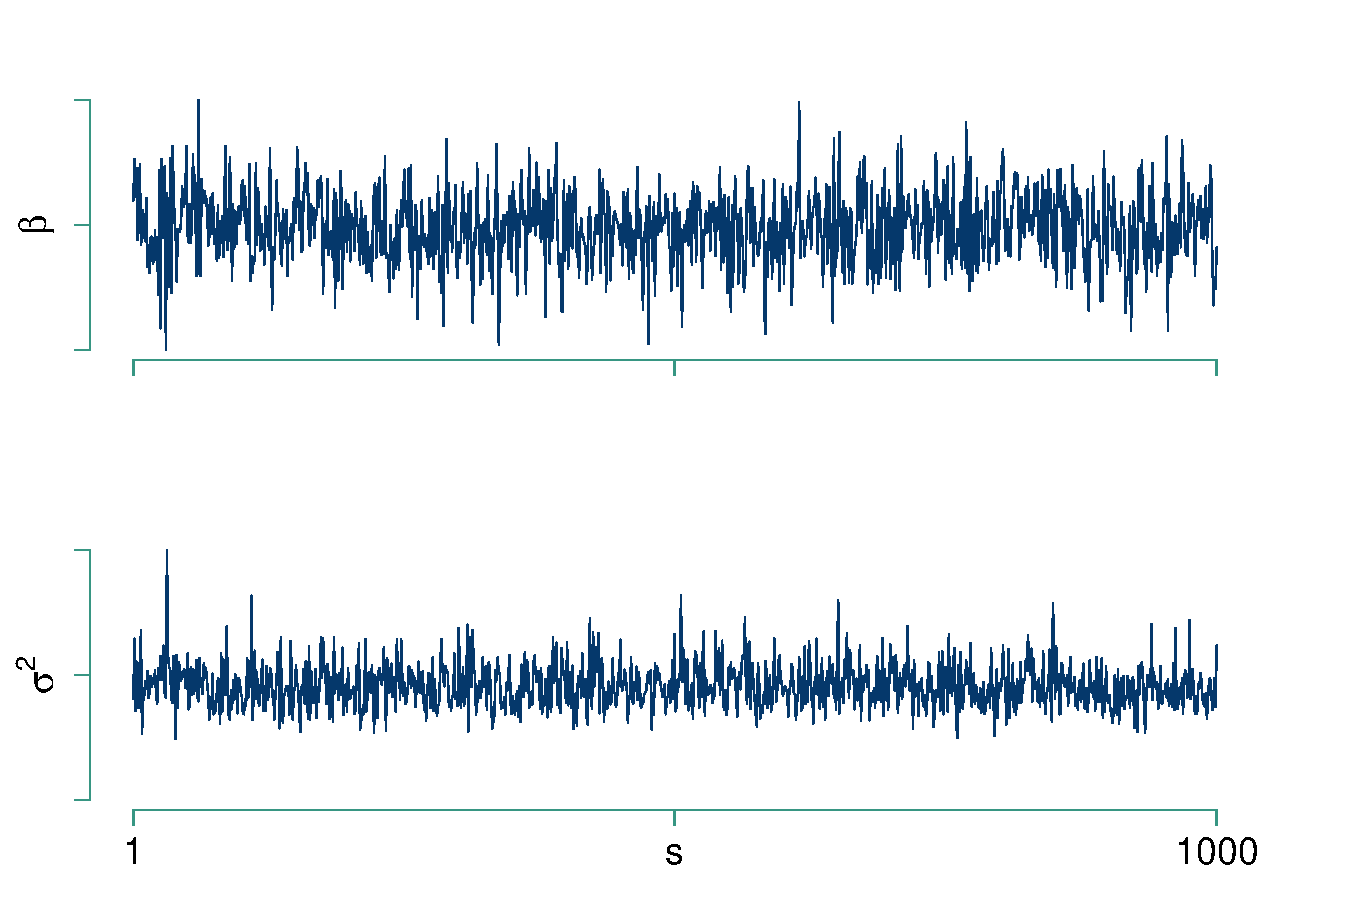
\includegraphics[scale=0.45]{./grphs/bs-trace.pdf}

\end{frame}
}



{\setbeamercolor{background canvas}{bg=mcxs4}
\begin{frame}{Gibbs sampler: illustration}
\centering
\textbf{Marginal posterior densities:} $p(\beta|Y,X)$ and $p\left(\sigma^2|Y,X\right)$\\
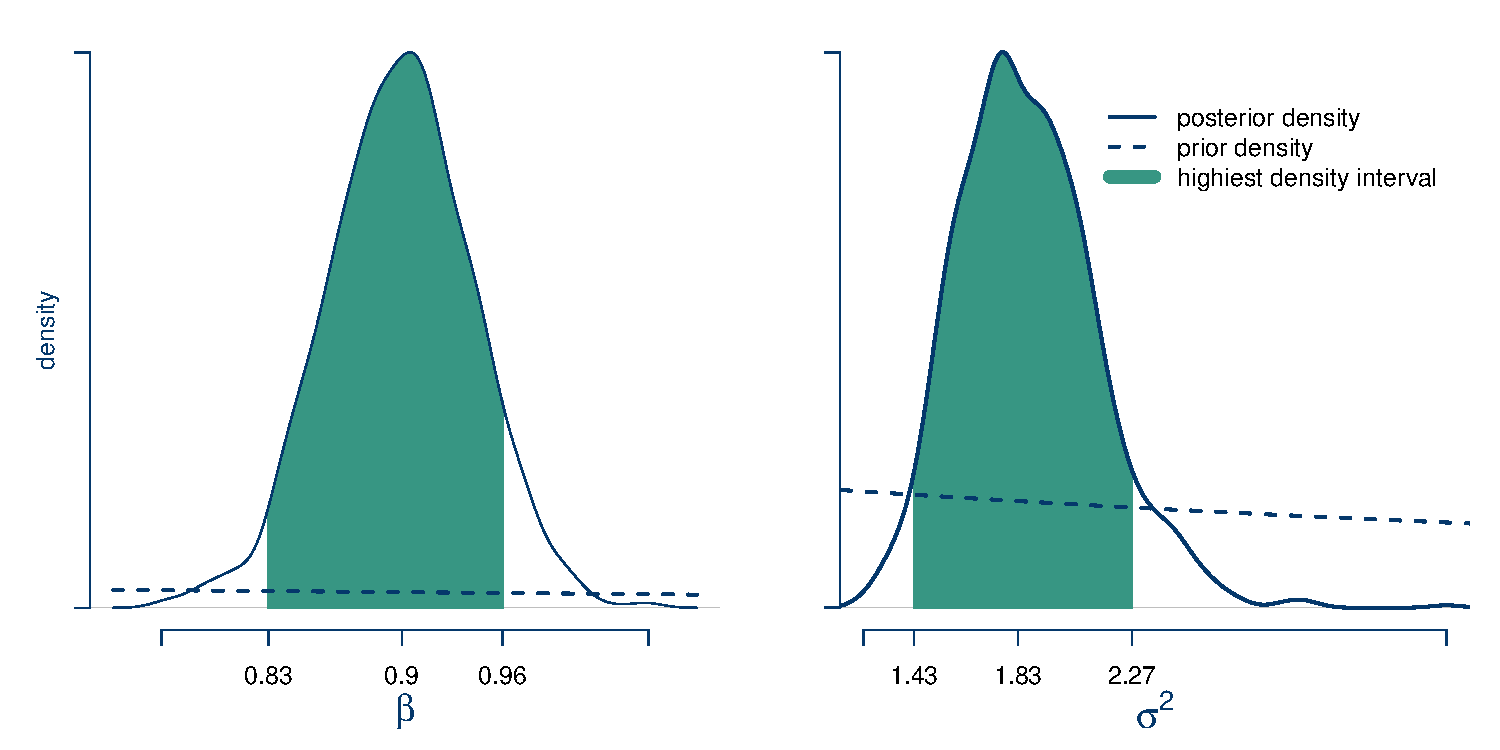
\includegraphics[scale=0.45]{./grphs/bs-marginal.pdf}

\end{frame}
}

{\setbeamercolor{background canvas}{bg=mcxs5}
\begin{frame}{Gibbs sampler: illustration}
\centering
\textbf{Joint posterior density:} $p\left(\beta,\sigma^2|Y,X\right)$\\
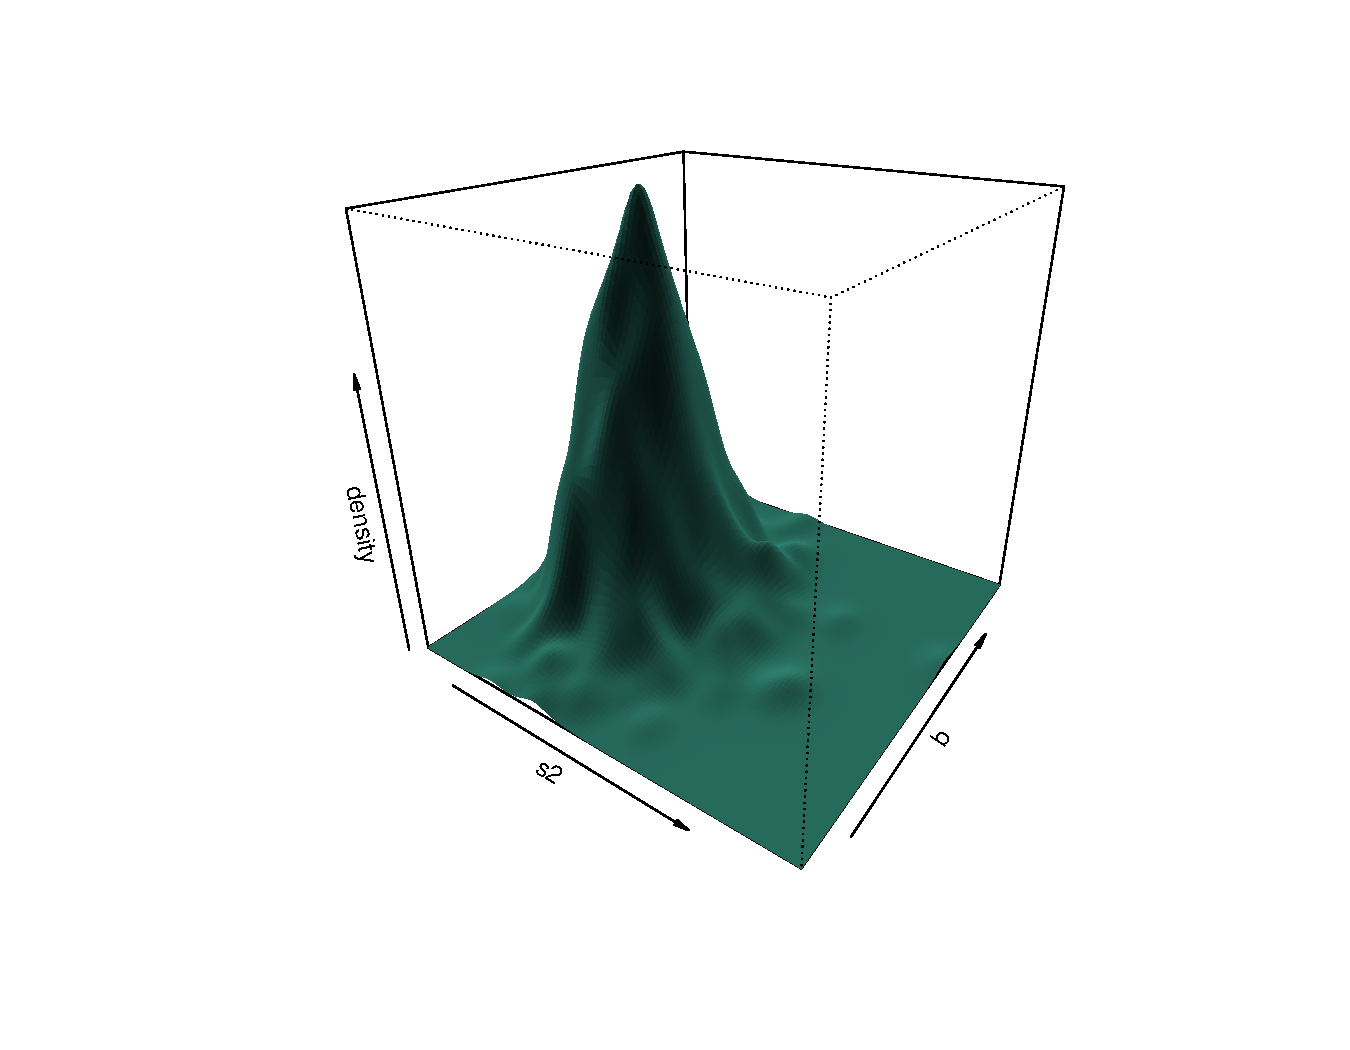
\includegraphics[scale=0.45, trim=0cm 3cm 0cm 2cm]{./grphs/bs-joint.pdf}

\end{frame}
}


{\setbeamercolor{background canvas}{bg=mcxs4}
\begin{frame}

\vspace{1cm} \textbf{\color{mcxs2}Numerical optimization}
\begin{description}
\item[Newton-Raphson] {\color{mcxs5}method}
\item[BHHH] {\color{mcxs5}method}
\end{description}

\bigskip\textbf{\color{mcxs2}Numerical integration}
\begin{description}
\item[Gibbs sampler]
\item[full conditional] {\color{mcxs5}posterior distributions}
\item[joint and marginal] {\color{mcxs5}posterior distributions}
\end{description}

\end{frame}
}


\end{document} 